\subsection{Paket: wrapfigure}

\begin{frame}[fragile]{wrapfigure}
Um Text um Bilder \enquote{herumfließen} zu lassen, benutzen wir das Paket \pkg{wrapfig}.

\begin{codeblock}
\begin{verbatim}
\usepackage{wrapfig}
\begin{document}
\begin{wrapfigure}{l}{6cm}
\includegraphics[width=0.5\textwidth]{xkcd1.png}
\end{wrapfigure}
\footnotesize \lipsum[1]

\end{document}
\end{verbatim}
\end{codeblock}
\pause
\end{frame}

\begin{frame}[fragile]{wrapfigure}
\begin{wrapfigure}
{l}
{6cm}
\includegraphics[width=0.5\textwidth]{images/xkcd1.png}
\end{wrapfigure}
\footnotesize \lipsum[1]
\end{frame}

\begin{frame}[fragile]{zu beachten bei wrapfigure}
\begin{codeblock}
\begin{verbatim}
\begin{wrapfigure}{l}{8cm}
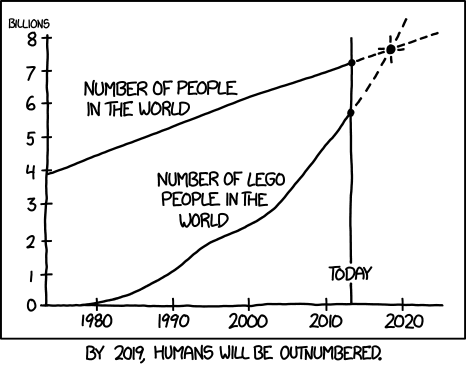
\includegraphics[width=0.5\textwidth]{xkcd.png}
\end{wrapfigure}
\end{verbatim}
\end{codeblock}

\begin{itemize}
 \item l=links ; 8cm=breite
 \item kein \textbackslash flushright, \textbackslash flushleft, \textbackslash centering im Text um das Bild. 
 (für das Bild selbst emfiehlt sich \textbackslash centering)
\end{itemize}
\end{frame}

